\chapter{Selection of protein}
\minitoc
\label{sec:selection}
\acrshort{DNA} to protein (cite Jacob \& Monod), is the first approximation on which to work, since the ability of cells to perform their function depends on the efficiency of the enzyme.
As such our proxy of fitness are trough proteins.

They are also analogous explanation between absolute and relative fitness \citep{Masel2016}.

Phylogenetic reconstruction seeks to infer past evolutionary history of life on Earth.
However, phylogeneticists are constrained to solely access present-day populations and extinct fossils.
One approach to circumvent this limitation is to study the evolution of molecular sequences backward in time, based on present-day molecular sequences.
In this molecular framework, evolution is generally seen as a stochastic process, and the interplay between point mutations and the selection of these mutations leads to substitutions in sequences over time.
Thus, molecular evolutionary biologists design substitution models of the sequences, and compute how likely they would observe the present-day molecular sequences, given a past-history scenario and a model of substitutions.\\
One major assumption of substitution models is independence between sites, meaning that any position of the sequence has its own independent evolutionary process and a substitution at one position does not affect the substitution process at other positions.
The motivation for this assumption is rooted in computational complexity rather than biological meaning, and crucially constrains the modeling process.\\
Under the site-independence assumption, the modeling approach essentially depends on the nature of the sequence under study.
For example, non-coding \acrshort{DNA} sequences are subject to very different evolutionary forces compared to protein-coding \acrshort{DNA} sequences, and must be addressed differently.
This review will focus on substitution models designed to address solely protein-coding \acrshort{DNA} sequences.
In such coding \acrshort{DNA} sequences the mutation process occurs at the \acrshort{DNA} level, but selection process occurs at the protein level in first approximation.
Thus studying protein coding \acrshort{DNA} sequences at the nucleotide level has a major shortcoming of not taking into account the true underlying selection process, which can lead to false conclusions in the phylogenetic reconstruction.\\
One simple approach to resolve this conflict is to study the evolutionary history of the protein instead of the \acrshort{DNA} sequence, meaning translating nucleotide sequences into amino-acid sequences, and design a model at the amino-acid level.
Equally, amino-acid substitution models have also the major shortcoming of not taking into account that the mutation process occurs at the nucleotide level.
Indeed, when studying sequences at the amino-acid level, the degeneracy of the genetic code leads to loss of information present in the mutated \acrshort{DNA} sequences, since the 61 codons are converted to the 20 amino-acids.\\

For protein-coding sequences, both \acrshort{DNA} and amino-acid substitution models fail to take into account either the selection or the mutation process.
These shortcomings are both addressed by codon models, basically combining the best of both models by studying nucleotides in triplets instead of independently.
In a codon substitution model, a mutation of a nucleotide in a triplet will either be synonymous, meaning not changing the translated amino-acid, or non-synonymous, meaning the translated amino-acid will be different.
The degeneracy of the genetic code is thus an advantage when one devises a model at the codon level in \acrshort{DNA} sequences.
One can identify the interplay between mutations acting at the \acrshort{DNA} level, and positive or negative selection acting at the protein level.
Thus, codon substitution models are crucial for a better modeling of the underlying evolution of protein-coding \acrshort{DNA} sequences, and consequently allow a better reconstruction of mutation, selection and demography.

\section{Insight from empirical data}
This section review the empirical evidence available, which will be important to keep in mind when the different models of selection will be 

\subsection{Substitution rate across genes}
Classical codon models estimate a parameter $\omega=d_N/d_S$, namely the ratio of the non-synonymous over the synonymous substitution rates \cite{Muse1994,Goldman1994}. In the so-called site-models, $\omega$ is allowed to vary across sites, either via a finite mixture \cite{Yang2001}, an infinite mixture \cite{Huelsenbeck2006}, or as random effects from a parametric distribution. In PhyloBayes, the latter option is used: site-specific $\omega^{(i)}$ are independent identically distributed from a gamma distribution \cite{lartillot_phylobayes_2013}. This implementation is used in this study to infer the distribution of $\omega$ across sites on empirical alignments. In a second step, the average over site is calculated, giving estimates of $\omega$ for each protein-coding sequences (see figure \ref{fig:codon_model}, left panel).
	
\begin{figure}[thbp]
	\begin{center}
		\includegraphics[width=\textwidth, page=2] {figures.pdf}
	\end{center}
	\caption{Substitution rate as a function of the selection coefficient.}
\end{figure}

\subsection{Substitution rate across sites}
Acknowledging the flaws of the initial codon models, It has been rapidly recognized that the parameter $\omega$ should not be estimated globally over the entire sequence [8]. The codons need to be separated into a finite number of different categories, with each category having its own $\omega$. In such so called sites models, the number of categories is specified before the analysis, and the category each codon falls into is estimated by maximum likelihood in so called finite mixture model (see box 1) [8–10]. In finite mixture models, the number of categories that increase the goodness of fit of the model can be asserted by the use of Akaike Information Criterion (AIC, see box 1). Using AIC, the computations usually estimate a number of categories tending to infinite, ultimately suggesting that each codon of the sequence should have its own $\omega$ [11]. In the Bayesian framework (see box 1), in contrast to maximum likelihood, the number of categories can be a variable. The flexibility of the computation mainly done by Markov Chain Monte Carlo (MCMC, see box 1) allows one to draw $\omega$ from an infinite mixture, usually using a Dirichlet process (see box 1), giving a posterior distribution of the parameter $\omega$ [12,13]. 

\subsection{Substitution rate across branches}
Which branches are 


\section{Generic model of selection}

\citet{Welch2008}

In Wilson \textit{et. al.}, the fitness effect of a mutation is drawn from a fitness distribution that is solely function of $\Ne$, meaning ${p_{\mathrm{fix}}}$ is independent from the current sequence state.
On the other hand, in the mutation-selection model proposed, the distribution of fitness effects is a function of the current state.


\section{Amino-acid propensities}

	In contrast, mutation-selection models assume that the protein-coding sequence (CDS) is at mutation-selection balance under a fixed fitness landscape, which is itself characterized by a fitness vector over the $20$ amino-acid at each site \cite{Yang2008, Halpern1998, Rodrigue2010}. Mathematically, the rate of non-synonymous substitution from codon $a$ to codon $b$ ($q_{a \mapsto b}^{(i)}$) at the $i^{\mathrm{th}}$ site of the sequence is equal to the rate of mutation at site $i$ ($\mu_{a \mapsto b}^{(i)}$) multiplied by the probability of fixation of the mutation ($p_{a \mapsto b}^{(i)}$) \cite{kimura_neutral_1983}. Crucially, the probability of fixation depends on the difference of fitness between the amino-acid encoded by the mutated codon ($f_b^{(i)}$) and the fitness of the amino-acid encoded by the original codon ($f_a^{(i)}$) of site $i$ \cite{wright_evolution_1931, fisher_genetical_1930}. Altogether, the rate of substitution from codon $a$ to $b$ at a given site $i$ is:
\begin{equation}
q_{a \mapsto b}^{(i)} = \mu_{a \mapsto b}^{(i)} \dfrac{\mathrm{ln}(f_b^{(i)} / f_a^{(i)})}{1 - f_b^{(i)} / f_a^{(i)}}.
\end{equation}

Fitting the mutation-selection model on a sequence alignment leads, via equation (1), to an estimation of the mutation rate matrix ($\mu^{(i)}$) as well as the fitness landscape of the protein ($f^{(i)}$) at each site $i$ of the sequence. From these parameters, one can compute $\omega_{0}^{(i)}$, the site-specific predicted rate of non-synonymous over synonymous substitution at the mutation-selection balance: 
\begin{equation}
\omega_{0}^{(i)} = \sum_{a \in  \mathcal{C}} \pi_a^{(i)}  \dfrac{\sum_{b \in  \mathcal{N}_a} q_{a \mapsto b}^{(i)}}{\sum_{b \in \mathcal{S}_a} q_{a \mapsto b}^{(i)}},
\end{equation}
where $\mathcal{C}$ is the set all the possible codons ($61$ by discarding stop codons), $\pi_a$ is the equilibrium frequency of codon $a$ at site $i$, and $\mathcal{N}_a$ (respectively $\mathcal{S}_a$) is the set of codons that are non-synonymous (respectively synonymous) to $a$  \cite{spielman_relationship_2015, rodrigue_site-heterogeneous_2014}. In a second step, the average over site is calculated, giving estimates of $\omega_0$ for each protein-coding sequences (see figure \ref{fig:codon_model}, right panel). \\

Under the assumption that the protein is under a \textit{nearly-neutral} regime,  the predicted $\omega_0$ (mutation-selection model) and the estimated $\omega$ (site-model) should be the same. But if this assumption is violated, and the protein is under adaptation then $\omega > \omega_0$.


In mutation-selection codon models, the probability of reaching fixation is different for any non-synonymous mutation.
More specifically, it will depend on the original amino-acid preference and the mutated amino-acid preference encoded by the codon.
From a dynamical perspective, a mutation on a codon with high preference (of the encoded amino-acid) will have a low probability of fixation, since the mutated codon will have a lower preference, and thus at equilibrium this low probability of fixation of the codon is compensated by a high frequency of the codon.
Essentially, at equilibrium the codon frequencies only fluctuate at the mutation-selection balance, and all the mutations are neutral on average, but slightly deleterious or advantageous, hence the name nearly-neutral models.\\
For evolutionary biologists, the assumption of equal amino-acid preference is equivalent to have a flat fitness landscape for all amino-acids, with neither a peak nor a valley.
In contrast, in nearly-neutral models, the amino-acids have a fitness landscape fixed in time, but that is not flat.
The difficulty and complexity of nearly-neutral models are to estimate the underlying amino-acid fitness landscape.
Moreover, nearly-neutral models consider multiplicative fitness across sites.

By modeling the population as a single sequence, we model a trajectory along a changing fitness landscape.
For each codon site, we compute the substitution rate to the $9$ neighboring codons (see equation 1)  
The time to the next substitution is exponentially distributed with parameter equal to the total rate.

\citep{Halpern1998a} 

Relative Evolutionary Rates in Proteins Are Largely Insensitive to the Substitution Model \citep{Spielman2018}.

Physicochemical Amino Acid Properties Better Describe Substitution Rates in Large Populations \citep{Weber2019}.

A new parameter-rich structure-aware mechanistic model for amino acid substitution during evolution \citep{Chi2018}.


\section{Protein folding}

ProtASR: An Evolutionary Framework for Ancestral Protein Reconstruction with Selection on Folding Stability \citep{Arenas2017}.


\subsubsection{Selection at the genome level}
Selfish genes

Variation of the adaptive substitution rate between species and within genomes \citep{Moutinho2019}.


